\chapter{Hardware}

\section{Board Overview}
The principal aim of the design was to develop an energy and reasonably cost-efficient wireless sensing platform, with easy expandability so as to support arbitrary sensor attachments. As a result, the designed board is a small, credit-card sized circuit board. Temperature, humidity, and ambient light-levels are measured on-board, while the remaining micro-controller general purpose input-output (GPIO) is broken out to a standard 0.1" pitch header. The board is based on the Texas Instruments CC3200 system-on-a-chip (SOC), containing an ARM-M4 MCU and an 802.11 WiFi radio.

\missingfigure{Board component-level block diagram}

The sensor node is designed to be small and non-invasive for easy deployment in residential and outdoor areas. The dimensions are sized to fit a standard Pelican 1010-series enclosure, so as to support an outdoor, battery-powered usage case. This case is rugged, waterproof, and made of transparent (optical and RF) polycarbonate.

\begin{table}[h]
\begin{tabular}{@{}l|lll@{}}
                    & Length (cm) & Width (cm) & Height (cm) \\ \midrule
Pelican 1010 Casing & 11.1        & 7.3        & 4.3         \\
Device PCB          & 10.5        & 6.5        &            
\end{tabular}
\caption{Enclosure and Board Dimensions}
\label{dimensions}
\end{table}

The system is designed to run autonomously with little interaction by the user. Accordingly, there are no buttons or switches on the board, however, if user interaction is required, they can be added to the 0.1" header. In order to facilitate easy development, however, an FTDI dual serial to USB chip is included on the board's footprint. One port connects to the CC3200 UART, and another to the CC3200 JTAG pins. This simplifies the development process as a JTAG probe set is no longer needed for in-circuit debugging and firmware flashing. The trace powering the FTDI adapter can be cut via jumper if the board is intended for long term battery operation, or the chip omitted entirely if large-scale production is anticipated.

The CC3200 SoC is over-specified for the base use-case, and contains spare computational and memory capacity. The internal ARM-M4 micro-controller runs at 80 MHz from a pair of external 32.768 kHz and 40 MHz crystal oscillators. The model specified in this design contains 128 kB of RAM and is run from an 8 MB serial flash module accessed over the SPI bus. As the current firmware load consumes around 40 kilobytes of RAM during regular operation, expanded functionality can easily be programmed in the future.

IEEE 802.11 (WiFI) was chosen for the wireless protocol. It was picked because WiFi is a ubiquitous wireless standard. As opposed to other protocols, it is extremely unlikely that additional routers or gateways would need to be purchased in order to connect the sensor board to the Internet. It is also amenable to easy network administration through well-known tools, as opposed to a custom or more esoteric protocol. However, 802.11 is not known for being especially power efficient nor is it a simple protocol. It has only recently been true that cheap 802.11 transceivers have been made available to the low-volume market. The power consumption of the 802.11 protocol is addressed in software via compression and aggregation of sensed data, and adjusting the duty cycle of the radio so that it spends most of the time idle. This trade-off is acceptable for this design as the majority of nodes are not battery-powered, and of those which are, most do not need to transmit data in real-time, allowing for long sleep periods.

\begin{table}[h]
\begin{tabular}{ll}
Voltage Supply           & 2.1 - 3.6V \\
Clock Frequency          & 80 MHz     \\
Maximum Current Draw     & 229 mA     \\
Sleep, Radio Idle Listen & 695 uA     \\
Sleep, All               & 129 uA \\
Hibernation              & 4 uA     \\
RAM (Code and Data)      & 128 kB     \\
Serial Flash Storage     & 8 MB		\\
Battery Capacity		 & 4000 mAH (2xAA)	      
\end{tabular}
\end{table}

\missingfigure{Photograph of PCB}

\section{Antenna Design}

The sensor board looks for three qualities in its antenna, in decreasing importance: cost, range, and compactness. Three antenna configurations were considered for the design. Planar inverted-F antennas (PIFA) are inexpensive and have a reasonable range, but are not as small as chip antennas. Ceramic chip antennas (CCA) are compact, but have poor range, and are expensive. Finally, externally mounted whip antennas have good range, but are also fairly expensive, and consume a large volume of space.

In this design, a PIFA was chosen. A PIFA has a simple structure, an omni-directional radiation pattern, and is very low-cost as it is fabricated as part of the PCB. It has an elliptical polarization, allowing it to receive both vertical and horizontally polarized waves\cite{huynh2000numerical}. This is important in an indoor environment as wireless waves often tend to become depolarized as they reflect off internal surfaces. In addition, one of the additional advantages of the PIFA is that it can be easily tuned by hand by fabricating the long arm of the F with excess length, and then scraping the excess surface copper until a good impedance match is obtained. For all these reasons, planar inverted-F antennas are extremely common in small electronic devices, and see common application in mobile handsets. Figure X shows the basic layout of a planar inverted-F antenna.

\begin{figure}[h]
\centering
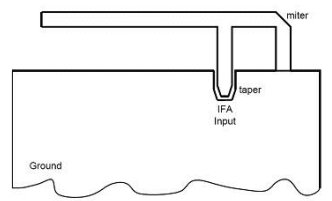
\includegraphics[width=0.5\linewidth]{images/pifa}
\caption[PIFA Layout]{A basic layout of a single band planar inverted-F antenna\cite{Rosu}.}
\label{fig:pifa}
\end{figure}


The PIFA has a few complexities in its design. Important factors are the size and aspect ratio of the F-structure, the height of the antenna over the ground plane, the position of the feed point, and the location of the shorting strap. These will all affect the electrical performance of the antenna.

A PIFA was designed and simulated in HFSS. The geometry is illustrated in Fig. \missingfigure{ HFSS PIFA PCB geometry}. The dielectric is standard 2-layer FR4 with a thickness of 1.6mm (63 mil) and 1 oz. copper traces and fills.

\section{Peripherals}
\subsection{Soil Moisture}

Zazueta, Fedro S., and Jiannong Xin. "Soil moisture sensors." Soil Sci 73 (1994): 391-401.

A ground-source heat pump (GSHP) was installed at ecoMOD 4. GSHPs transfer heat between the ground and a conditioned room or facility using electrical energy. Heat pump efficiency is inversely proportional to the temperature differential between the source and destination. As opposed to traditional electric air conditioners and heaters which use the ambient air temperature as the source, GSHPs source from the ground, whose temperature is approximately equal to the mean annual temperature year round, or around 50-60 degrees Fahrenheit, leading to generally better efficiency. GSHP installation and use disturbs the soil temperature, so in order to effectively calculate pump efficiency, the surrounding soil temperature and moisture content (which heavily determines the heat capacity of the surrounding soil) must be known.

Soil moisture can be measured in many different ways. However, only a few of these techniques lend themselves to automated electronic sensing, and the most common and widely available are based around either resistive or capacitive sensor methods. 

Capacitive methods involve measuring the dielectric capacitance between two electrodes. This is usually done by measuring the impedance at a specific frequency. The measured impedance is not linearly proportional to the amount of water present, and varies according to the composition and temperature of the measured soil. Therefore, for absolute precision, the sensor must be calibrated against a representative sample of soil and the temperature measured as well. When calibrated, the measurement is generally highly precise and can be measured instantaneously. Capacitive sensors are generally more expensive due to the more precise electronics required and calibration needed for accurate results.

\missingfigure{Irrometer Watermark Sensor}

Resistive techniques measure the DC resistance of a given volume of soil. The most common way of measuring this is by burying a porous gypsum block into the ground along with two electrodes, and allowing the block to come to hydrostatic equilibrium with the surrounding soil. This process usually takes two to three hours, which can also be seen after a rainstorm or other meteorological event. They are electronically simpler and cheaper to manufacture than capacitive sensors, which is an important consideration for their most common use, large-scale agricultural deployments. For many applications, individual block calibration can be ignored, since the gypsum medium is of a well-known composition and possesses a consistent resistivity. However, for long term measurement accuracy, the gypsum block must be continually recalibrated, as soil ions and salts can migrate into the gypsum block matrix, affecting the block resistance.

\missingfigure{Vegetronix}

\subsection{Ambient Humidity and Temperature}

\subsection{Ambient Light}



